\section{The Hard Disk Drive Scaling Trilemma}
\label{sec:trilemma}

\subsection{Hard Disk Drives and the Trilemma}
\label{sec:hard-disk-drives}

The first hard drive was released in 1956 by IBM and could hold less than $5$MB of data. Since then an increase in areal density (information stored per unit area) of order $10^{7}$ has been achieved by scaling down the area used to store each bit (made possible by improvements in the read heads, write heads and various other hard drive parts)\cite{Stefanita2008}. However the ability to simply scale down in this way is coming to an end due to the so called ``trilemma'' of magnetic data storage\cite{Chan2010}. The trilemma (extended from dilemma) refers to the relationship between three crucial aspects of magnetic data storage: the signal to noise ratio (or SNR), thermal stability and writability. Current hard disk drives store data using the magnetic orientations of magnetic grains. The combination of many grains within predefined area constitutes a single bit.

Increasing the areal density requires a decrease in the size taken up by each bit. The signal to noise ratio of read outs from the disk increases if the number of grains per bit is reduced because the bit edges become fuzzy. To avoid degrading the signal to noise ratio when reducing the size of each bit the size of grains should be decreased instead of the number of grains per bit.\cite{McDaniel2005} If the size of grains is reduced too far (without any other changes) then the energy barrier preventing the grain from flipping magnetisation becomes close to the thermal energy at the operating temperature (typically just above room temperature). This results in grains spontaneously flipping magnetisation, hence the bits that these grains represent are unstable and the disk becomes unsuitable for use as a long term storage device. The limit on areal density due to these thermal effects is sometimes known as the \emph{superparamagnetic limit}.

One solution to this problem is to use a material with a higher anisotropy (i.e. a material that requires more energy per unit volume to change its magnetisation direction), thus increasing the energy barrier needed to flip the magnetisation of a grain. However, this also makes the grains harder to flip when writing to them, requiring a stronger write head field.

Until now the write heads have been able to cope with any increases in write field required and so thermal stability has been retained while decreasing grain size.\cite{McDaniel2005} However there are material limitations on the maximum possible field generated by the write head\cite{Richter2007a} and the actual write field within the disk is further limited by geometrical effects. Hence, to continue improving the areal density of disks a new paradigm appears to be needed.

A potential solution is to use \emph{bit patterned media} \cite{Terris2006} (BPM) and/or \emph{heat assisted magnetic recording}\cite{Kryder2008} (HAMR). Bit pattern media uses a single, comparatively large, magnetic domain to store each bit, avoiding the thermal instability problem of very small magnetic domains. A comparison of bit patterned media with conventional media is illustrated in Figure~\ref{fig:Layouts-for-magnetic}. In heat assisted recording the area being written to is heated up (e.g. using a laser), briefly reducing the anisotropy and allowing writing to take place even in very high anisotropy materials. These two solutions could potentially be used together to allow areal densities up to $\sim10^{3}$ times that of current hard drives.\cite{McDaniel2005}

\begin{figure}[!ht]
  \center
  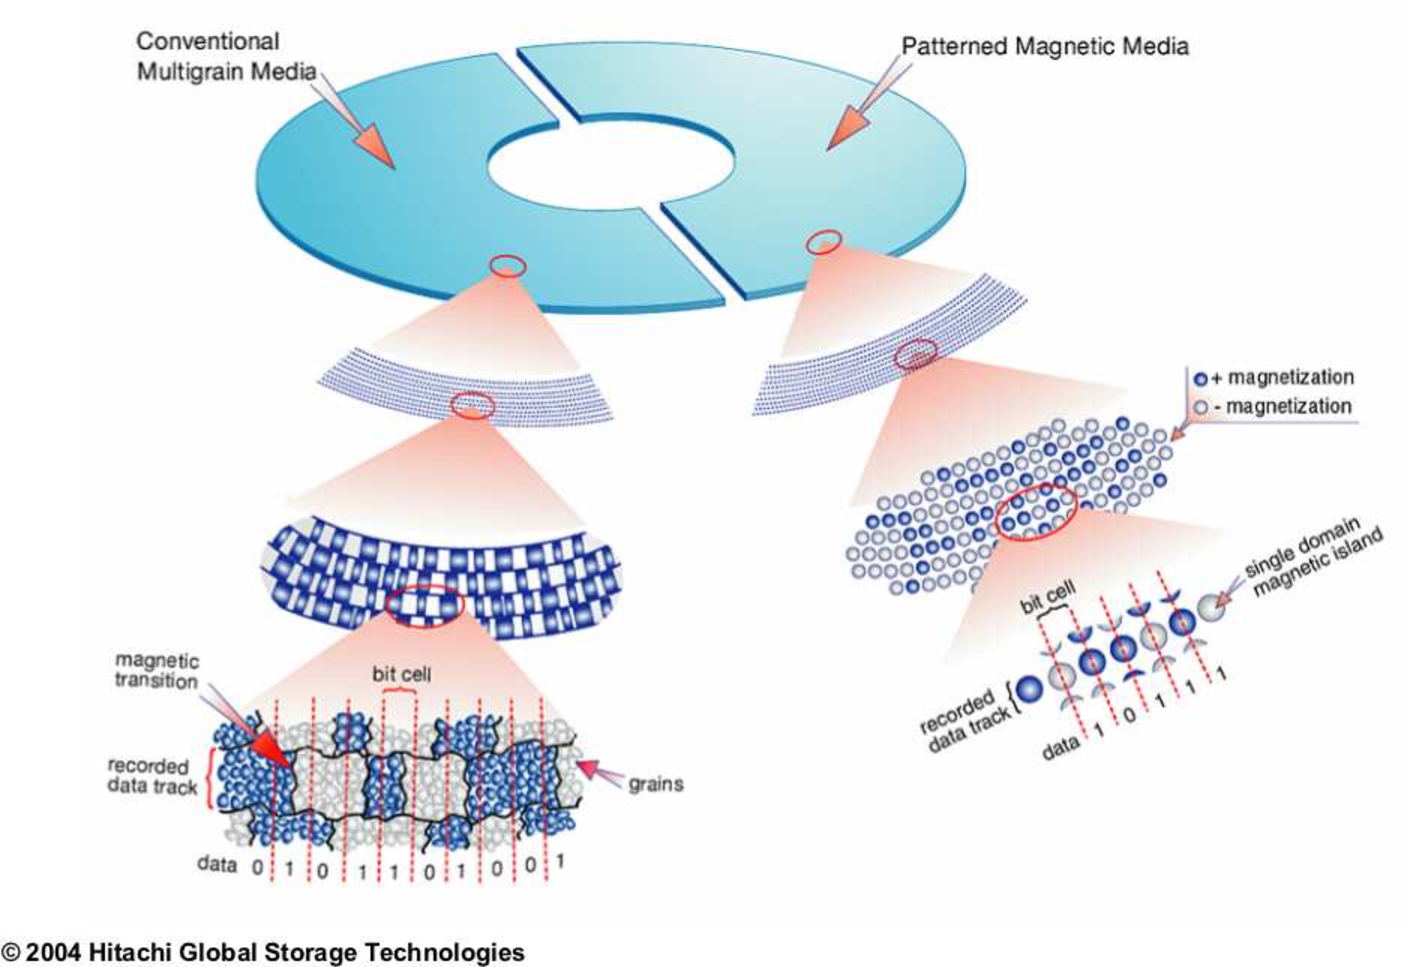
\includegraphics[width=0.75\textwidth]{./images/conventional_vs_pattern_media}
  \caption{Different media types for magnetic data storage. Conventional multigrain media is
    the layout used in current hard disk drives. Bit pattern media is a potential new layout which could allow for further scaling up of data density.
    \cite{conventional_vs_patterned_media} \label{fig:Layouts-for-magnetic}}
\end{figure}

\subsection{Mathematical Description of the Trilemma}

We present a very simple description of how the areal density of a disk depends on the three factors mentioned in Section~\ref{sec:hard-disk-drives}.

The anisotropy of a material refers to its preference for magnetisation along one axis (typically in either direction), often called the \emph{easy axis}. There are various types of anisotropy, caused by different effects. The most important is magnetocrystalline anisotropy which is caused by the crystal structure of the material affecting the electrons resulting in preferred spin directions.\cite{Getzlaff2008}

In the absence of an applied field the magnetocrystalline anisotropy
causes an energy barrier between opposite magnetisations. A useful
quantity is $K$, the energy per unit volume required to overcome
this energy barrier and flip the magnetisation direction. When writing
to a grain the applied field must overcome the energy barrier before
switching the magnetisation. Thus an applied field

\begin{equation}
\Happ > \dfrac{2K}{\mu_{0}M_s},
\label{eq:43}
\end{equation}

is needed, where $M_s$ is the saturation magnetisation of the material and $\mu_0 = 4 \pi \E{-7} \text{N A}^{-2}$ is the magnetic constant.\cite{McDaniel2005}

A good measure of thermal stability is the ratio between the energy required to
flip the magnetisation of a grain, $KV$ (where $V$ is the grain volume) and the
thermal energy $k_{B}T$ ($k_{B}$ is Boltzmann's constant, $T$ is the temperature
in Kelvin)

\begin{equation}
  \eta_{0}=\dfrac{KV_{grain}}{k_{B}T}.\label{eq:eta}
\end{equation}
For acceptable thermal stability with a typical distribution of grain
volumes $\eta_0 \gtrsim 60$ is required.\cite{McDaniel2005}

For a disk with $N$ grains per bit, grain thickness $\delta$ and packing
fraction $p$ (the ratio of magnetic to non-magnetic areas of the
disc) the area per bit is
\[
A_{bit}=\dfrac{N}{p}\cdot A_{grain}=\dfrac{N}{p}\cdot\dfrac{V_{grain}}{\delta}
\]

The areal density $D$ of a disk is the inverse of the area per bit,
hence
\[
D=A_{bit}^{-1}=\dfrac{p\delta}{NV_{grain}}.
\]

Finally, substituting in $V_{grain}=\dfrac{\eta_{0}k_{B}T}{K}$ from \eqref{eq:eta} gives
\begin{equation}
D=\dfrac{p\delta}{k_{B}T}\cdot\dfrac{K}{N\eta_{0}}.\label{eq:AD}
\end{equation}


From \eqref{eq:AD} we see which factors can be scaled to increase the areal
density of a disk, but some of these factors can be immediately ruled
out. Cooling of hard drives (i.e. reduction of $T$) is probably not an option
for any real world applications because the small improvement in stability (and
hence areal density) that could be gained is vastly outweighed by inconvenience
and cost of cooling. The track depth $\delta$ cannot be increased beyond twice
the bit length because multiple domains will start to form in the vertical
direction \cite{McDaniel2005} and also reducing the track depth can degrade
performance\cite{Litvinov2002}. Reducing the packing fraction can only lead to a
small areal density increase because most of the disk already consists of
magnetic material.

This leaves the anisotropy $K$, the number of grains per bit $N$ and the thermal
stability $\eta_{0}$ as possible scaling factors.  However, the signal to noise
ratio depends on the sharpness of the boundaries between bits, which is
dependant on the number of grains per bit. Fewer grains per bit results in a
rougher bit boundary and hence more noise. Additionally the thermal stability is
proportional to the grain volume. Hence we are left with a trade off between
signal to noise ratio, thermal stability and writability: the trilemma.

Bit pattern media sidesteps the problem by removing the dependence
of signal to noise ratio on $N$ and reducing $N$ to one. The signal
to noise ratio is then dominated by how well the actual island locations
correspond to their theoretical locations, which is determined by
the manufacturing process. It has been demonstrated that the signal
to noise ratio for bit pattern media can be at least as low as in
traditional media.\cite{Moritz2004}

Thermally assisted recording allows for a large increase in stability while maintaining writability because the value of $K$ at high temperatures (i.e. when writing) is typically far lower than at room temperature (i.e. when thermal stability is needed).

The model presented above is a vast simplification of the actual magnetisation process. For example, inter-grain effects, time dependence and grain shape have all been ignored. However it is still useful to see that there is a trade-off between the various factors and to understand how bit pattern media and heat assisted magnetic recording can help circumvent some of the problems.


%%% Local Variables:
%%% mode: latex
%%% TeX-master: "main"
%%% End:
